%=============================================================================
%  PRIMORDIA — Technical report & user manual
%  Interactive Graphics course
%  Compile with:  pdflatex report.tex   (twice, for the table of contents)
%=============================================================================
\documentclass[11pt,a4paper]{article}

\usepackage[T1]{fontenc}
\usepackage[utf8]{inputenc}
\usepackage[english]{babel}
\usepackage[a4paper,margin=2.4cm]{geometry}
\usepackage{amsmath,amssymb}
\usepackage{graphicx}
\usepackage{booktabs}
\usepackage{longtable}
\usepackage{array}
\usepackage{enumitem}
\usepackage[protrusion=true,expansion=false]{microtype}
\usepackage{xcolor}
\usepackage{listings}
\usepackage{tcolorbox}
\usepackage{caption}
\usepackage{float}
\usepackage{fancyhdr}
\usepackage{titlesec}
\usepackage{tikz}
\usepackage{pgfplots}
\pgfplotsset{compat=1.16}
\usetikzlibrary{positioning,arrows.meta,fit,backgrounds}
\usepackage[colorlinks=true,linkcolor=accent!70!black,urlcolor=accent!70!black,
            citecolor=accent!70!black]{hyperref}

%--- colours -----------------------------------------------------------------
\definecolor{accent}{RGB}{22,140,125}
\definecolor{accent2}{RGB}{70,110,190}
\definecolor{codebg}{RGB}{246,247,249}
\definecolor{codekw}{RGB}{150,40,120}
\definecolor{codecm}{RGB}{110,120,130}
\definecolor{rulegray}{RGB}{200,205,212}

%--- headers -----------------------------------------------------------------
\pagestyle{fancy}
\fancyhf{}
\renewcommand{\headrulewidth}{0.4pt}
\fancyhead[L]{\small\textsc{Primordia} — 3D Emergence Lab}
\fancyhead[R]{\small\thepage}

%--- section styling ---------------------------------------------------------
\titleformat{\section}{\Large\bfseries\color{accent!75!black}}{\thesection}{0.7em}{}
\titleformat{\subsection}{\large\bfseries}{\thesubsection}{0.6em}{}
\titleformat{\subsubsection}{\normalsize\bfseries}{\thesubsubsection}{0.5em}{}

%--- code listings -----------------------------------------------------------
\lstdefinestyle{js}{
  language=Java,
  basicstyle=\ttfamily\footnotesize,
  keywordstyle=\color{codekw}\bfseries,
  commentstyle=\color{codecm}\itshape,
  stringstyle=\color{accent2},
  backgroundcolor=\color{codebg},
  frame=leftline,
  framerule=1.2pt,
  rulecolor=\color{accent!60},
  xleftmargin=10pt,
  framexleftmargin=6pt,
  breaklines=true,
  showstringspaces=false,
  columns=fullflexible,
  morekeywords={let,const,function,of,in,new,return,for,if,else,while,var},
}
\lstset{style=js}

\newcommand{\code}[1]{\texttt{\small #1}}
\newcommand{\file}[1]{\texttt{\small\color{accent!70!black}#1}}

\newtcolorbox{notebox}[1]{colback=accent!5,colframe=accent!55,
  title=#1,fonttitle=\bfseries\small,boxrule=0.7pt,left=6pt,right=6pt,top=4pt,bottom=4pt}

\newcommand{\keys}[1]{\textsf{\small\fbox{#1}}}

%=============================================================================
\begin{document}

%--- title page --------------------------------------------------------------
\begin{titlepage}
\centering
\vspace*{2.2cm}

{\color{accent}\rule{\textwidth}{1.6pt}}
\vspace{0.7cm}

{\Huge\bfseries PRIMORDIA\par}
\vspace{0.4cm}
{\LARGE A 3D Emergence Laboratory\par}
\vspace{0.5cm}
{\large Two-scale particle life with Barnes--Hut gravity\\and a piloted articulated creature\par}

\vspace{0.5cm}
{\color{accent}\rule{\textwidth}{1.6pt}}

\vspace{1.6cm}
{\large\textbf{Technical Report and User Manual}\par}
\vspace{0.4cm}
{\normalsize Interactive Graphics course\par}

\vspace{2.4cm}

\begin{tabular}{rl}
\textbf{Application type} & Real-time interactive 3D web application\\[3pt]
\textbf{Environment}      & WebGL via three.js (r128), plain ES6 JavaScript\\[3pt]
\textbf{External assets}  & None --- all geometry, textures and\\
                          & animation are generated procedurally\\[3pt]
\textbf{Entry point}      & \file{index.html}\\
\end{tabular}

\vfill
{\small A real-time simulation in which two force laws acting at different spatial
scales --- short-range, type-dependent ``chemistry'' and long-range,
mass-dependent gravity --- produce emergent structure that the user can inspect,
perturb, and swim through with a hand-animated creature.\par}
\vspace{1cm}
\end{titlepage}

\tableofcontents
\newpage

%=============================================================================
\section{Introduction}
%=============================================================================

\subsection{What the application is}

\textsc{Primordia} is a real-time, interactive 3D laboratory for \emph{emergence}: the
phenomenon in which a large number of agents obeying very simple local rules produce
complex global structure that was never explicitly programmed. The user does not build
the structures --- the user changes the rules, and then watches, steers and disturbs
whatever the rules produce.

The simulation superimposes two force laws that act at deliberately different spatial
scales, which is the conceptual core of the project:

\begin{itemize}[leftmargin=1.4em,itemsep=3pt]
  \item \textbf{Short-range ``chemistry''.} Every particle carries a discrete
        \emph{type} (a colour). An \emph{asymmetric} matrix $A$ specifies how strongly
        type $i$ is attracted to or repelled by type $j$ within a small radius
        $r_{\max}$. Because $A_{ij} \neq A_{ji}$ in general, the system is
        non-conservative and produces the chasing, cycling and self-propelling
        behaviour characteristic of \emph{particle life}. This term is responsible for
        local structure: cells, membranes, filaments, worms.
  \item \textbf{Long-range gravity.} Every particle also carries a mass derived from
        its radius, and attracts every other particle with an inverse-square law.
        This term is responsible for global structure: collapse, clumping, orbits,
        spiral arms.
\end{itemize}

Neither force alone is novel. Their superposition is what makes the application
interesting to explore: gravity assembles the coarse skeleton, chemistry decorates it,
and the two fight each other in ways that are genuinely difficult to predict from the
parameter values alone.

Naive evaluation of both laws would cost $O(N^2)$ per frame, which is far too slow for
the $1{,}000$--$3{,}000$ particles we target at 60\,Hz. Each law is therefore
accelerated by the data structure that suits its own spatial scale --- a uniform grid
for the short-range term, a Barnes--Hut octree for the long-range one. Section
\ref{sec:technical} describes both in detail.

Finally, the soup is inhabited. A hierarchical, self-animated creature (the
\emph{Grazer}) is built as a real three.js scene graph with four articulated legs
running a procedural gait. The user pilots it with the keyboard; it is a solid obstacle
that particles bounce off, and it emits its own local force field, so it is a physical
participant in the simulation rather than a decorative overlay.

\subsection{Design goals}

\begin{enumerate}[leftmargin=1.6em,itemsep=3pt]
  \item \textbf{Everything procedural.} No mesh files, no image files, no imported
        animation clips. Every vertex, every texel and every joint angle in the
        application is computed in JavaScript at run time. This was a self-imposed
        constraint, and it shapes many of the technical decisions in this report.
  \item \textbf{Real-time at meaningful $N$.} The simulation must stay interactive
        with thousands of mutually interacting particles, which rules out the naive
        all-pairs approach and motivates the two acceleration structures.
  \item \textbf{Everything is live.} No parameter change requires a reload. Particle
        count, type count, world size, and the rule matrix can all be edited while the
        simulation runs, and the affected buffers and data structures are rebuilt
        in place.
  \item \textbf{The rules are visible.} The user can display the octree subdivision,
        the gravitational field as animated streamlines, and a wireframe lattice of
        space that deforms under mass and under the user's own interventions. The
        acceleration structure is not hidden --- it is part of the exhibit.
  \item \textbf{Zero-friction deployment.} Opening \file{index.html} from disk must be
        sufficient. No build step, no bundler, no local server, no \code{npm install}.
\end{enumerate}

\subsection{How to read this document}

Section \ref{sec:environment} describes the execution environment; Section
\ref{sec:external} lists everything used but not written by us; Section
\ref{sec:architecture} explains the code structure; Section \ref{sec:technical} is the
technical core (physics, acceleration structures, rendering, the creature); Section
\ref{sec:interactions} documents every implemented interaction; Section
\ref{sec:manual} is the user manual proper, and can be read on its own by someone who
only wants to run the application.

%=============================================================================
\section{Description of the environment used}
\label{sec:environment}
%=============================================================================

\subsection{Rendering environment}

The application is a \textbf{client-side web application} rendering through
\textbf{WebGL}, accessed via the \textbf{three.js} library (revision 128) rather than
through raw WebGL calls. Concretely:

\begin{itemize}[leftmargin=1.4em,itemsep=3pt]
  \item The rendering context is created by \code{THREE.WebGLRenderer}, which selects
        a WebGL\,2 context when the browser provides one and silently falls back to
        WebGL\,1 otherwise. The application uses no feature that requires WebGL\,2, so
        it runs correctly on both.
  \item The renderer is configured with \code{antialias:\,true} (MSAA on the default
        framebuffer) and \code{powerPreference:\,'high-performance'}, which asks the
        browser to select the discrete GPU on dual-GPU laptops.
  \item The device pixel ratio is clamped, \code{setPixelRatio(Math.min(devicePixel\-Ratio,2))}.
        On a high-DPI display an unclamped ratio would quadruple the fragment load for
        a barely perceptible gain; the clamp is a deliberate, and very effective,
        performance decision.
  \item Output is written in sRGB (\code{outputEncoding = THREE.sRGBEncoding}) so that
        lighting is composited in linear space and converted once at the end, which is
        what makes the emissive teals and pinks read correctly rather than washing out.
\end{itemize}

We chose three.js over hand-written WebGL deliberately. The project's intellectual
content is the \emph{simulation} --- the force laws, the grid, the octree, the
articulated model and the gait --- and all of that is written from scratch. Delegating
context creation, shader compilation and matrix bookkeeping to a mature library let us
spend the available time on the parts of the project that are actually ours. Nothing in
the physics or in the model hierarchy is inherited from the library: three.js is used
as a rendering back end and a scene-graph container, not as a simulation framework.

\subsection{Language and execution model}

The application is written in \textbf{plain ES6+ JavaScript}. There is no TypeScript,
no JSX, no transpilation and no bundling. The consequences are worth stating explicitly
because they influenced the code structure:

\begin{itemize}[leftmargin=1.4em,itemsep=3pt]
  \item \textbf{No build step.} The source that ships is the source that runs, which
        makes the project trivial to inspect and to grade.
  \item \textbf{Classic scripts, not ES modules.} The JavaScript files are loaded as
        ordinary \code{<script src=\ldots>} tags in dependency order and share a single
        global lexical scope. This is a conscious trade-off: ES modules would give
        explicit import graphs, but browsers refuse to load modules over the
        \code{file://} protocol for security reasons, which would force every user to
        start a local web server. Classic scripts keep the ``double-click
        \file{index.html}'' promise. The dependency order is documented in
        \file{index.html} and in each file's header comment (Section
        \ref{sec:architecture}).
  \item \textbf{Single-threaded.} The whole simulation runs on the main thread, inside
        the animation-frame callback. There are no Web Workers. This bounds
        the achievable particle count, and Section \ref{sec:limitations} discusses it as
        the first candidate for future work.
\end{itemize}

\subsection{Runtime requirements and platform support}

\begin{table}[H]
\centering
\small
\begin{tabular}{@{}ll@{}}
\toprule
\textbf{Requirement} & \textbf{Detail}\\
\midrule
Browser        & Any modern browser with WebGL: Chrome, Firefox, Edge, Safari\\
GPU            & Any GPU capable of WebGL\,1; integrated graphics are sufficient\\
Network        & Needed \emph{once}, to fetch three.js from the CDN (see \S\ref{sec:external})\\
Server         & Not required --- the \code{file://} protocol works\\
Installation   & None\\
Input          & Mouse + keyboard (full feature set); touch (camera only)\\
\bottomrule
\end{tabular}
\caption{Runtime requirements.}
\end{table}

\noindent The application is responsive: below a viewport width of 560\,px the control
console expands to full width and the HUD is hidden, and the camera accepts one-finger
drag (orbit) and two-finger pinch (zoom). Creature piloting and the drag tools require a
keyboard and mouse respectively, so a desktop browser is the intended target.

%=============================================================================
\section{External libraries, tools and models}
\label{sec:external}
%=============================================================================

This section lists exhaustively everything in the delivered project that was
\textbf{not} written by the team.

\subsection{Libraries}

\begin{table}[H]
\centering
\small
\renewcommand{\arraystretch}{1.25}
\begin{tabular}{@{}p{2.5cm}p{1.4cm}p{4.2cm}p{6.2cm}@{}}
\toprule
\textbf{Library} & \textbf{Version} & \textbf{Source} & \textbf{What it is used for}\\
\midrule
three.js & r128 & \code{cdnjs.cloudflare.com} \newline (single \code{<script>} tag) &
The \emph{only} runtime dependency. Used for: WebGL context and render loop
(\code{WebGLRenderer}); scene graph (\code{Scene}, \code{Group}, \code{Object3D}) and
its transform composition; \code{PerspectiveCamera} and projection; primitive geometry
generators (\code{SphereGeometry}, \code{CylinderGeometry}, \code{BoxGeometry},
\code{TorusGeometry}, \code{EdgesGeometry}); the standard PBR material
(\code{MeshStandardMaterial}) and its shaders; \code{InstancedMesh} for batched particle
drawing; lights; \code{CanvasTexture}; \code{BufferGeometry} for the line
visualisations; and the math types (\code{Vector2/3}, \code{Color}, \code{Plane},
\code{Raycaster}).\\
\bottomrule
\end{tabular}
\caption{Third-party libraries. There is exactly one.}
\end{table}

\noindent That is the complete list. No UI framework (React, Vue), no control-panel
library (dat.GUI, lil-gui, Tweakpane), no physics engine (cannon.js, ammo.js), no math
library (gl-matrix), no utility library (lodash), no bundler (webpack, Vite, Rollup),
no package manager, no CSS framework. The control console, the attraction-matrix
editor, the HUD and the camera controller were all written for this project; in
particular we did \emph{not} use three.js's own \code{OrbitControls}, because it ships
as a separate add-on file and our camera has to interoperate with the poke tools, which
share the same mouse buttons.

\subsection{Models, meshes and animation}

\begin{notebox}{None.}
There are no imported 3D models, no \code{.obj}/\code{.gltf}/\code{.fbx} files, no
rigs, and no imported animation clips or keyframe data anywhere in the project.
\end{notebox}

\noindent Every piece of geometry in the scene is assembled at run time from
three.js's parametric primitive generators:

\begin{itemize}[leftmargin=1.4em,itemsep=2pt]
  \item \textbf{Particles} --- one \code{SphereGeometry(1, 10, 8)}, drawn $N$ times by
        an \code{InstancedMesh}.
  \item \textbf{The Grazer} --- roughly two dozen spheres, cylinders and a torus,
        composed into a hierarchy of \code{Group}s (Section \ref{sec:creature}).
  \item \textbf{The boundary cage} --- \code{EdgesGeometry} of a \code{BoxGeometry}.
  \item \textbf{Octree, field and lattice visualisations} --- \code{BufferGeometry}
        objects whose vertex buffers we fill by hand every frame.
\end{itemize}

\noindent The Grazer's walk cycle is likewise not an imported clip: it is a closed-form
function of a phase accumulator, evaluated per leg per frame (Section
\ref{sec:gait}).

\subsection{Textures}

\begin{notebox}{None imported.}
All three texture maps are \textbf{painted procedurally into an off-screen
\code{<canvas>}} at start-up and uploaded via \code{THREE.CanvasTexture}.
\end{notebox}

\noindent Three $128\times128$ maps are generated (\S\ref{sec:textures}): an
\emph{albedo} map (radial gradient plus 900 random speckles), a \emph{normal} map (70
overlapping radial gradients perturbing the tangent-space normal), and a
\emph{roughness} map (1{,}400 random grey squares). Generating them costs a few
milliseconds once and keeps the project asset-free.

\subsection{Fonts}

The CSS font stacks name Inter, SF Mono, JetBrains Mono and Roboto Mono, but no font is
\emph{fetched}: there is no \code{@font-face} rule and no Google Fonts link. Each stack
ends in a generic family (\code{system-ui}, \code{sans-serif}, \code{monospace}), so the
named fonts are used only if the user's machine already has them and the OS default is
used otherwise. The application therefore carries no font dependency.

\subsection{Conceptual credits}

The short-range rule model is our implementation of the well-known \emph{particle life}
/ ``Clusters'' idea popularised by Jeffrey Ventrella and by Hunar Ahmad
(\code{hunar4321}). We credit the idea in the application footer. No code was taken:
the original demonstrations are 2D, use all-pairs evaluation, and have neither variable
mass nor gravity. Our contribution is the extension to 3D, the addition of a
mass-dependent long-range term with a Barnes--Hut octree, the uniform-grid acceleration
of the short-range term, the live visualisations, and the piloted articulated creature.

The Barnes--Hut algorithm itself is the standard published method \cite{barneshut}; the
implementation in \file{js/octree.js} is ours.

\subsection{Development tools}

\begin{table}[H]
\centering
\small
\begin{tabular}{@{}ll@{}}
\toprule
\textbf{Tool} & \textbf{Role}\\
\midrule
Text editor              & Writing the source\\
Browser developer tools  & Debugging, profiling, frame timing\\
\LaTeX                   & This document\\
\bottomrule
\end{tabular}
\caption{Development tools. No compiler, bundler, package manager or asset pipeline is
part of the workflow.}
\end{table}

%=============================================================================
\section{Software architecture}
\label{sec:architecture}
%=============================================================================

\subsection{File organisation}

The project is deliberately flat and readable: one HTML entry point, one stylesheet,
ten JavaScript files, each with a single responsibility.

\begin{center}
\small
\begin{tabular}{@{}p{4.2cm}p{1.3cm}p{9.4cm}@{}}
\toprule
\textbf{File} & \textbf{Lines} & \textbf{Responsibility}\\
\midrule
\file{index.html}        & 45  & Markup for the console, HUD and pilot hint; declares script load order.\\
\file{css/style.css}     & 128 & All presentation: console panel, HUD, sliders, toggles, matrix grid, responsive rules.\\
\midrule
\file{js/config.js}      & 54  & \code{CFG} (every tunable), \code{Poke} (intervention state), \code{PALETTE}. Single source of truth.\\
\file{js/scene.js}       & 88  & Renderer, camera object, lights, boundary cage, poke marker, procedural textures.\\
\file{js/particles.js}   & 56  & Particle buffers, seeding, attraction matrix, \code{InstancedMesh}.\\
\file{js/creature.js}    & 163 & Grazer model hierarchy, procedural gait, keyboard piloting.\\
\file{js/grid.js}        & 38  & Uniform grid (counting sort) and the particle-life force kernel.\\
\file{js/octree.js}      & 124 & Barnes--Hut octree: build, mass/COM pass, traversal.\\
\file{js/simulation.js}  & 282 & The integrator and the three debug visualisations; mesh sync.\\
\file{js/camera.js}      & 71  & Orbit/pan/zoom, screen-to-world unprojection, mouse and touch bindings.\\
\file{js/ui.js}          & 293 & Widget factory, control console, matrix editor, impulses, presets.\\
\file{js/main.js}        & 57  & Frame loop, HUD, resize handling, bootstrap.\\
\bottomrule
\end{tabular}
\end{center}

\subsection{Dependency order}

Because the files are classic scripts sharing one global scope, \textbf{load order is
part of the design}. Each file may use anything declared in the files above it. The
order encoded in \file{index.html} is exactly the dependency graph:

\begin{center}
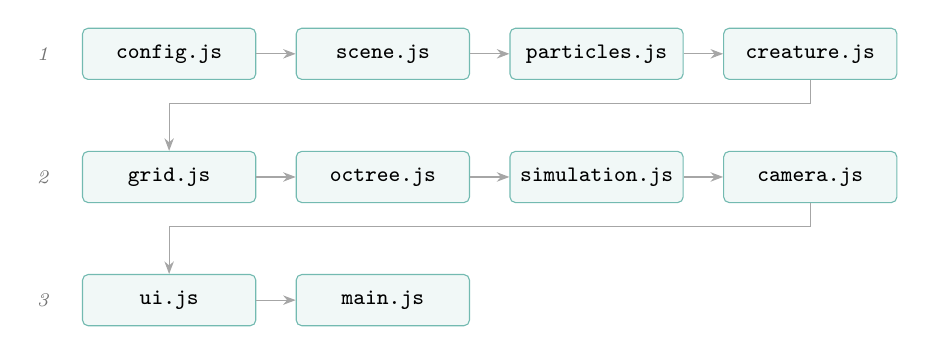
\begin{tikzpicture}[
  node distance=5mm,
  box/.style={draw=accent!60,fill=accent!6,rounded corners=2pt,minimum height=6.5mm,
              minimum width=22mm,font=\footnotesize\ttfamily,align=center},
  lay/.style={font=\scriptsize\itshape,color=black!55},
  ar/.style={-{Stealth[length=1.6mm]},draw=black!35}
]
\node[box] (cfg) {config.js};
\node[box,right=of cfg] (scn) {scene.js};
\node[box,right=of scn] (par) {particles.js};
\node[box,right=of par] (cre) {creature.js};

\node[box,below=9mm of cfg] (grd) {grid.js};
\node[box,right=of grd] (oct) {octree.js};
\node[box,right=of oct] (sim) {simulation.js};
\node[box,right=of sim] (camf) {camera.js};

\node[box,below=9mm of grd] (ui) {ui.js};
\node[box,right=of ui] (mn) {main.js};

\node[lay,left=3mm of cfg] {1};
\node[lay,left=3mm of grd] {2};
\node[lay,left=3mm of ui] {3};

\draw[ar] (cfg)--(scn); \draw[ar] (scn)--(par); \draw[ar] (par)--(cre);
\draw[ar] (cre.south) -- ++(0,-3mm) -| (grd.north);
\draw[ar] (grd)--(oct); \draw[ar] (oct)--(sim); \draw[ar] (sim)--(camf);
\draw[ar] (camf.south) -- ++(0,-3mm) -| (ui.north);
\draw[ar] (ui)--(mn);
\end{tikzpicture}
\end{center}

\noindent \file{config.js} comes first because every other file reads \code{CFG};
\file{main.js} comes last because it bootstraps. Only \file{main.js} executes
significant work at load time --- the others declare state and functions, with a handful
of self-contained initialisation calls (building the cage, generating the textures,
attaching input listeners).

The bootstrap is five lines and shows the whole start-up sequence:

\begin{lstlisting}
allocParticles(N); allocOctree(); rebuildGridDims();
randomizeMatrix(); seedParticles(); buildMesh(); buildCreature(); buildLattice(); buildPanel();
applyCam();
requestAnimationFrame(frame);
\end{lstlisting}

\subsection{Data layout: structure of arrays}
\label{sec:soa}

Particles are \textbf{not} objects. There is no \code{Particle} class and no array of
instances. State is held in parallel typed arrays --- a \emph{structure of arrays}
(SoA) layout:

\begin{lstlisting}
function allocParticles(n){
  px=new Float32Array(n); py=new Float32Array(n); pz=new Float32Array(n);
  vx=new Float32Array(n); vy=new Float32Array(n); vz=new Float32Array(n);
  ptype=new Uint8Array(n); psize=new Float32Array(n); pmass=new Float32Array(n);
}
\end{lstlisting}

This is the single most important performance decision in the project, for three
reasons:

\begin{enumerate}[leftmargin=1.6em,itemsep=3pt]
  \item \textbf{Cache locality.} The inner loop of \code{simulate()} streams
        sequentially through \code{px}, \code{py}, \code{pz}. With an array of objects
        each access would chase a pointer into a scattered heap allocation; here the
        next value needed is almost always in the cache line already fetched.
  \item \textbf{No garbage collector pressure.} Typed arrays are allocated once, at
        start-up or on a population change. In steady state the simulation allocates
        \emph{nothing} per frame, so the GC never runs, so there are no collection
        pauses --- which in an animation is the difference between smooth and stuttering.
  \item \textbf{Predictable types.} \code{Float32Array} elements cannot be boxed or
        change representation, which lets the JIT emit unboxed floating-point code for
        the whole inner loop.
\end{enumerate}

The same discipline is applied to the octree (\S\ref{sec:octree}), which is a pooled SoA
structure of thirteen typed arrays rather than a tree of node objects, and to the
gravity field samples.

%=============================================================================
\section{Technical aspects}
\label{sec:technical}
%=============================================================================

\subsection{Scene, camera and lighting}

The scene is a dark volume with exponential fog (\code{FogExp2}, density $0.006$)
matching the background colour $\mathtt{0x05070d}$, so distant particles dissolve into
the background instead of ending abruptly at the far plane --- a cheap and effective
depth cue in a scene that is otherwise a cloud of similar-looking spheres.

The camera is a \code{PerspectiveCamera} with a $55^\circ$ vertical field of view and a
near/far range of $0.5$ to $2000$ world units. It is never manipulated directly; it is a
dependent variable of the orbit state described in \S\ref{sec:orbit}.

Lighting is a deliberately conventional four-light rig plus two accent lights:

\begin{center}
\small
\begin{tabular}{@{}llll@{}}
\toprule
\textbf{Light} & \textbf{Type} & \textbf{Colour / intensity} & \textbf{Purpose}\\
\midrule
\code{ambient} & Ambient     & \code{0x33405a}, 0.55 & Lifts shadowed sides out of black\\
\code{sun}     & Directional & \code{0xbcd3ff}, 0.85 & Key light, cool daylight from above\\
\code{rim}     & Directional & \code{0x2a4a7a}, 0.50 & Back/rim light, separates silhouettes\\
\code{p1}      & Point       & \code{0x37e0c8}, 1.60 & Teal accent; orbits the origin each frame\\
\code{p2}      & Point       & \code{0xff6bb0}, 1.20 & Pink accent, static\\
\bottomrule
\end{tabular}
\end{center}

\noindent The two point lights have finite range (260 and 220 units) and physical
quadratic decay. \code{p1} is animated on a slow circle of radius 40:

\begin{lstlisting}
p1.position.set(Math.sin(t*0.3)*40, 30, Math.cos(t*0.3)*40);
\end{lstlisting}

\noindent Its moving highlight sweeping across a static clump is often the clearest
visual signal that a structure is three-dimensional rather than a flat sprite cloud. The
accent pair can be toggled off from the console.

\subsection{Procedural texture generation}
\label{sec:textures}

Three maps are painted into $128\times128$ off-screen canvases at start-up and wrapped
in \code{CanvasTexture}:

\begin{itemize}[leftmargin=1.4em,itemsep=3pt]
  \item \textbf{Albedo} --- an off-centre radial gradient (white $\to$ light grey $\to$
        blue-grey) with 900 random white speckles at $\le 10\%$ alpha. It is kept
        \emph{light} on purpose: the per-instance colour multiplies this map, so a dark
        albedo would mute the type colours. Tagged \code{sRGBEncoding}, since it is
        colour data rather than measured data.
  \item \textbf{Normal} --- filled with the neutral tangent-space normal
        $(128,128,255)$, then overlaid with 70 radial gradients of random radius whose
        red and green channels are randomly offset by up to $\pm 60$. Each blob is a
        small bump. Applied at \code{normalScale} $=(0.6,0.6)$ on particles and a much
        subtler $(0.25,0.25)$ on the creature body.
  \item \textbf{Roughness} --- mid-grey with 1{,}400 random $2\times2$ squares of
        varying value, giving micro-variation in specular response so that a clump of
        identically-coloured particles does not look like a single moulded object.
\end{itemize}

Total cost is a few milliseconds once at start-up, and the reward is that the project
ships with no image files at all.

\subsection{Particle representation and instanced rendering}

Each particle $i$ has position $\mathbf{x}_i$, velocity $\mathbf{v}_i$, a type
$t_i \in \{0,\dots,T-1\}$, a radius $s_i$ and a mass $m_i$. Radii are drawn at seed time
from a distribution deliberately skewed toward small values:

\begin{lstlisting}
const base=0.55, sv=CFG.sizeVariance;
const s = base*(1-sv) + base*sv*(0.4 + Math.pow(Math.random(),2.2)*3.4);
psize[i]=s;
pmass[i]=s*s*s;   // volume-like mass
\end{lstlisting}

The exponent $2.2$ biases \code{Math.random()} toward zero, so the population is mostly
small particles with a few large ones --- and since $m_i = s_i^3$, those few large ones
carry disproportionate gravitational mass. This is what makes the gravity presets
interesting: a handful of heavy seeds act as attractors around which the light majority
organises, exactly as in the astrophysical case being evoked. The
\code{sizeVariance} slider interpolates from a uniform population ($sv=0$) to a highly
varied one ($sv=1$).

Initial positions are uniform \emph{by volume} inside a sphere of radius
$0.7\,h$, which requires the cube-root inversion of the radial CDF:

\begin{lstlisting}
const L=Math.sqrt(a*a+b*b+cc*cc)||1;      // random direction
const r=Math.cbrt(Math.random())*R;       // cbrt => uniform density, not centre-heavy
px[i]=a/L*r; py[i]=b/L*r; pz[i]=cc/L*r;
\end{lstlisting}

\noindent Omitting the \code{cbrt} would concentrate particles near the centre, seeding
a gravitational collapse before the user has touched anything.

\paragraph{Rendering.} All $N$ particles are drawn by a single
\code{THREE.InstancedMesh} --- one sphere geometry, one material, one draw call. Two
details matter:

\begin{itemize}[leftmargin=1.4em,itemsep=2pt]
  \item The instance matrix buffer is flagged \code{DynamicDrawUsage}, telling the
        driver the buffer changes every frame so it can choose the right memory
        residency.
  \item Per-instance colour is written once per type change via \code{setColorAt}, not
        per frame. Only the transform buffer is re-uploaded each frame, by
        \code{syncMesh()}.
\end{itemize}

\begin{lstlisting}
function syncMesh(){
  for(let i=0;i<N;i++){
    dummy.position.set(px[i],py[i],pz[i]);
    dummy.scale.setScalar(psize[i]);
    dummy.updateMatrix();
    mesh.setMatrixAt(i, dummy.matrix);
  }
  mesh.instanceMatrix.needsUpdate=true;
}
\end{lstlisting}

\noindent A single reused \code{Object3D} (\code{dummy}) composes each matrix, so this
function allocates nothing. The sphere is only $10\times8$ segments --- 80 faces. At
$N=3000$ that is a quarter of a million triangles, which is comfortable; at
$32\times16$ it would be a million, which is not. The normal map restores the surface
detail that the coarse tessellation gives up.

\subsection{Short-range chemistry: the force law}
\label{sec:chem}

Let $\hat r = r/r_{\max}$ be the normalised distance between two particles, $\beta$ the
repulsion-core fraction, and $a = A_{t_i t_j}$ the (signed) attraction coefficient. The
scalar force profile is piecewise linear:

\begin{equation}
F(\hat r, a) =
\begin{cases}
\dfrac{\hat r}{\beta} - 1, & 0 \le \hat r < \beta \quad\text{(universal repulsion)}\\[10pt]
a\left(1 - \dfrac{\big|\,2\hat r - 1 - \beta\,\big|}{1-\beta}\right), & \beta \le \hat r < 1 \quad\text{(typed interaction)}\\[10pt]
0, & \hat r \ge 1 \quad\text{(no interaction)}
\end{cases}
\end{equation}

\begin{center}
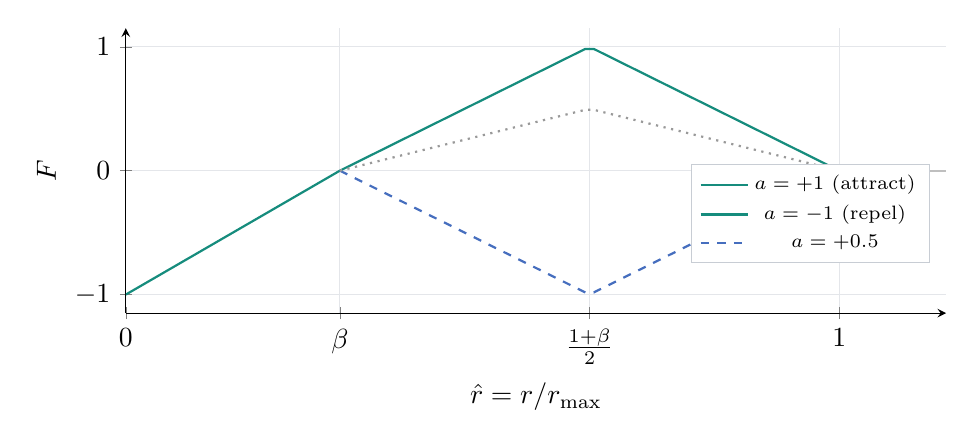
\begin{tikzpicture}
\begin{axis}[
  width=12cm, height=5.2cm,
  xlabel={$\hat r = r/r_{\max}$}, ylabel={$F$},
  xmin=0, xmax=1.15, ymin=-1.15, ymax=1.15,
  axis lines=left, xtick={0,0.3,0.65,1}, xticklabels={$0$,$\beta$,$\frac{1+\beta}{2}$,$1$},
  ytick={-1,0,1}, grid=major, grid style={rulegray!50},
  every axis plot/.append style={thick},
  legend style={font=\scriptsize,at={(0.98,0.35)},anchor=east,draw=rulegray},
]
% repulsion core: r/beta - 1  for 0..0.3
\addplot[accent,domain=0:0.3,samples=2]{x/0.3-1};
% attractive a=1: peak at (1+beta)/2 = 0.65
\addplot[accent,domain=0.3:1,samples=60]{1*(1-abs(2*x-1-0.3)/(1-0.3))};
\addlegendentry{$a=+1$ (attract)}
% repulsive a=-1
\addplot[accent2,dashed,domain=0.3:1,samples=60]{-1*(1-abs(2*x-1-0.3)/(1-0.3))};
\addlegendentry{$a=-1$ (repel)}
\addplot[black!40,dotted,domain=0.3:1,samples=60]{0.5*(1-abs(2*x-1-0.3)/(1-0.3))};
\addlegendentry{$a=+0.5$}
\addplot[black!25,domain=1:1.15,samples=2]{0};
\end{axis}
\end{tikzpicture}
\captionof{figure}{The particle-life force profile, drawn with $\beta=0.3$. Below
$\beta$ the force is a type-independent repulsion that reaches $-1$ at contact; between
$\beta$ and $1$ it is a triangular lobe scaled by the matrix entry $a$, peaking at
$\hat r = (1+\beta)/2$; beyond $r_{\max}$ it is exactly zero, which is what makes the
uniform grid valid.}
\end{center}

Three properties of this law carry the whole design:

\begin{enumerate}[leftmargin=1.6em,itemsep=3pt]
  \item \textbf{The repulsion core is universal.} For $\hat r < \beta$ the profile does
        not depend on $a$ at all. Every particle pushes every other particle away at
        very close range, regardless of type, which is what prevents the entire
        population from collapsing to a single point under mutual attraction. The
        \code{beta} slider is therefore effectively an incompressibility control.
  \item \textbf{The interaction is compactly supported.} $F$ is exactly zero beyond
        $r_{\max}$ --- not asymptotically small, but zero. This is the precondition for
        the uniform grid: a particle can only be influenced by particles within
        $r_{\max}$, so a grid with cell size $r_{\max}$ makes the $3\times3\times3$
        neighbourhood a \emph{complete} search domain, not an approximation.
  \item \textbf{The matrix is asymmetric.} $A_{ij}$ and $A_{ji}$ are independent, so
        Newton's third law is deliberately violated. If red chases green while green
        flees red, the pair self-propels and momentum is not conserved. This is
        physically false and behaviourally essential: it is the source of every
        chasing, cycling and locomotive pattern in the system.
\end{enumerate}

The accumulated short-range acceleration on particle $i$ is

\begin{equation}
\mathbf{a}_i^{\text{chem}} = r_{\max}\,k \!\!\sum_{j \,:\, r_{ij} < r_{\max}} \!\! F\!\left(\frac{r_{ij}}{r_{\max}},\, A_{t_i t_j}\right) \hat{\mathbf{d}}_{ij},
\qquad \hat{\mathbf{d}}_{ij} = \frac{\mathbf{x}_j - \mathbf{x}_i}{r_{ij}}
\end{equation}

\noindent where $k$ is the \code{forceStrength} slider. Note the $r_{\max}$ factor: it
keeps the effective force scale roughly constant as the user drags the interaction
radius, so changing $r_{\max}$ changes the \emph{geometry} of the patterns without
simply making everything more violent.

\subsection{Uniform grid acceleration}
\label{sec:grid}

Evaluating the sum above naively is $O(N^2)$. Since the kernel has compact support, we
bin particles into a uniform grid of cell size $r_{\max}$ and search only the 27
neighbouring cells.

The grid resolution adapts to both the world size and the interaction radius, capped to
bound memory:

\begin{lstlisting}
gN = Math.max(1, Math.floor(world / CFG.rMax));
gN = Math.min(gN, 64);          // <= 262144 cells
gCells = gN*gN*gN;
\end{lstlisting}

\paragraph{Counting-sort build.} The grid is rebuilt from scratch every frame --- there
is no incremental update, which would be more complex and, at these particle counts,
slower. The build is a three-pass counting sort into flat typed arrays, and allocates
nothing:

\begin{lstlisting}
function buildGrid(){
  cellCount.fill(0);
  for(let i=0;i<N;i++){ const c=cellIndex(px[i],py[i],pz[i]); cellOf[i]=c; cellCount[c]++; }
  let acc=0;
  for(let c=0;c<gCells;c++){ cellStart[c]=acc; acc+=cellCount[c]; }
  cellStart[gCells]=acc;
  const cursor=cellStart.slice(0,gCells);
  for(let i=0;i<N;i++){ const c=cellOf[i]; sortedIdx[cursor[c]++]=i; }
}
\end{lstlisting}

\noindent Pass 1 histograms the cells, pass 2 turns the histogram into a prefix sum, and
pass 3 scatters particle indices into \code{sortedIdx} so that the members of cell $c$
occupy the contiguous slice \code{sortedIdx[cellStart[c] .. cellStart[c+1])}. The whole
build is $O(N + \text{cells})$, and the resulting layout means the inner loop walks
neighbours contiguously in memory.

The query then decomposes the linear cell index back into $(i_x,i_y,i_z)$ and sweeps the
27-cell neighbourhood; the HUD reports the number of pairs actually evaluated per frame,
which typically sits between one and two orders of magnitude below $N^2$.

\paragraph{Complexity.} With roughly constant density, the expected cost is $O(N)$ ---
each particle examines a bounded number of neighbours --- against $O(N^2)$ for the naive
version. At $N=3000$ that is the difference between $9\times10^6$ pair tests per frame
and a few tens of thousands.

\subsection{Long-range gravity: Barnes--Hut octree}
\label{sec:octree}

Gravity has infinite support: every particle attracts every other, so the grid trick
does not apply and an exact evaluation is irreducibly $O(N^2)$. We use the Barnes--Hut
approximation \cite{barneshut}: a distant \emph{group} of particles is replaced by a
single pseudo-particle at the group's centre of mass.

\paragraph{Structure.} The octree is a pooled SoA structure --- thirteen typed arrays
indexed by node id, not a graph of objects:

\begin{lstlisting}
maxNodes = Math.max(256, N*4+64);
nCx,nCy,nCz  : Float32Array(maxNodes)   // node centre
nHalf        : Float32Array(maxNodes)   // half-width
nMass        : Float32Array(maxNodes)   // total mass
nComX/Y/Z    : Float32Array(maxNodes)   // centre of mass
nBody        : Int32Array(maxNodes)     // body index if leaf, -1 otherwise
nInternal    : Uint8Array(maxNodes)     // 0 = leaf, 1 = internal
nDepth       : Uint8Array(maxNodes)
nChild       : Int32Array(maxNodes*8)   // 8 child ids, -1 = absent
\end{lstlisting}

\noindent Allocation happens once, on a population change. Rebuilding the tree every
frame then costs \emph{zero} allocations: \code{buildOctree()} simply resets
\code{nodeCount=0} and re-uses the pool. Children are created lazily by \code{childOf()},
so an empty region of space costs nothing.

\paragraph{Build.} Bodies are inserted one at a time into a root cube covering the whole
world. The insertion loop handles the standard subtle case --- inserting into an
occupied leaf requires pushing the existing body down as well, and if both bodies land
in the same octant the process must recurse:

\begin{lstlisting}
if(nInternal[node]===0){
  if(nBody[node]===-1){ nBody[node]=i; return; }        // empty leaf: done
  const e=nBody[node]; nBody[node]=-1; nInternal[node]=1;   // occupied: subdivide
  if(nHalf[node]<0.02) return;                          // coincident-body guard
  const ce=childOf(node, octant(node,px[e],py[e],pz[e])); nBody[ce]=e;
  const ci=childOf(node, octant(node,px[i],py[i],pz[i]));
  if(ci===ce){ node=ci; continue; }                     // same octant: go deeper
  nBody[ci]=i; return;
}
\end{lstlisting}

\noindent The \code{nHalf < 0.02} guard is essential: two exactly (or nearly)
coincident bodies would otherwise subdivide forever, hanging the browser. Below that
cell size we drop the body from the tree for that frame --- an invisible error at this
scale, and a hard bound on depth. A second guard caps the insertion loop at 64
iterations.

\paragraph{Mass pass.} A post-order recursion aggregates mass and centre of mass:
\begin{equation}
M_{\text{node}} = \sum_{c \in \text{children}} M_c,
\qquad
\mathbf{X}_{\text{node}} = \frac{1}{M_{\text{node}}}\sum_{c \in \text{children}} M_c\,\mathbf{X}_c
\end{equation}

\paragraph{Traversal and the opening criterion.} For each particle the tree is walked
with an explicit stack (an \code{Int32Array(4096)} reused across calls --- recursion
here would mean a JS call frame per node and no way to bound depth). A node of width $s$
at distance $d$ is accepted as a single pseudo-particle when

\begin{equation}
\frac{s}{d} < \theta
\qquad\Longleftrightarrow\qquad
s^2 < \theta^2 d^2
\end{equation}

\noindent and is otherwise opened and its children pushed. The squared form is what the
code evaluates, avoiding a square root per node test:

\begin{lstlisting}
const s = nHalf[node]*2;
if(s*s < theta2*d2){ /* far enough: treat as one body */ }
else { /* push the 8 children */ }
\end{lstlisting}

\noindent The contribution of an accepted node is the softened inverse-square law

\begin{equation}
\mathbf{a}_i \mathrel{+}= \frac{G\,M_{\text{node}}\,(\mathbf{X}_{\text{node}} - \mathbf{x}_i)}{\left(\|\mathbf{X}_{\text{node}} - \mathbf{x}_i\|^2 + \varepsilon^2\right)^{3/2}}
\end{equation}

\noindent where $\varepsilon$ is the \code{softening} parameter. Softening is not
cosmetic: without it, two particles passing close together produce an acceleration
$\propto 1/r^2 \to \infty$, and with a finite time step they are slingshotted to
infinity, destroying the simulation. The $\varepsilon^2$ term bounds the force at
$G M/\varepsilon^2$ and keeps the integrator stable. Note that $\varepsilon$ is included
in the \emph{force} evaluation but not in the \emph{opening} test, which is the standard
formulation.

\paragraph{$\theta$ and the accuracy/speed trade-off.} $\theta$ is exposed as a slider
because it \emph{is} the algorithm's central dial:

\begin{center}
\small
\begin{tabular}{@{}lll@{}}
\toprule
$\theta$ & \textbf{Behaviour} & \textbf{Cost}\\
\midrule
$\to 0$   & Every node is opened; degenerates to exact all-pairs & $O(N^2)$\\
$0.5$     & High accuracy, more nodes visited & Slower\\
$0.8$     & Default; the usual accuracy/speed compromise & $O(N\log N)$\\
$1.6$     & Aggressive approximation, visible clumping artefacts & Fastest\\
\bottomrule
\end{tabular}
\end{center}

\noindent The HUD's octree node count makes the trade-off legible in real time: raising
$\theta$ visibly cuts the number of nodes visited and raises the frame rate.

A second entry point, \code{gravityAccelAt(root,x,y,z,out)}, evaluates the same field at
an \emph{arbitrary} point rather than at a particle. It is identical except that it
omits the self-exclusion test, and it is what drives the field-arrow and lattice
visualisations (\S\ref{sec:viz}).

\subsection{Integration and stability}

The two force terms, plus the creature field and the user's intervention field, are
summed per particle and integrated with \textbf{semi-implicit (symplectic) Euler} ---
velocity is updated first, then position is updated using the \emph{new} velocity, which
is markedly more stable for orbital motion than explicit Euler at the same cost.

Friction is applied as an exponential decay expressed through a \emph{half-life} rather
than a raw coefficient:

\begin{equation}
\mu = 2^{-\Delta t / T_{1/2}},
\qquad
\mathbf{v} \leftarrow \mu\,\mathbf{v} + \mathbf{a}\,\Delta t
\end{equation}

\begin{lstlisting}
const mu = Math.pow(0.5, dt/CFG.frictionHalfLife);
\end{lstlisting}

\noindent This formulation is framerate-independent by construction --- a half-life of
$45$\,ms means velocity halves every $45$\,ms of \emph{simulated} time regardless of how
many steps that took --- and it gives the user a control with a physical meaning
("motion halves in this long") instead of an arbitrary number.

Three further stability measures:

\begin{itemize}[leftmargin=1.4em,itemsep=3pt]
  \item \textbf{Time-step clamp.} \code{simulate(1/60 * Math.min(2, rdt*60))} caps the
        step at $1/30$\,s, and the raw frame delta is itself clamped at $50$\,ms.
        After a stall (the user switches tabs and returns) a huge $\Delta t$ would blow
        the simulation apart; the clamp trades a moment of slow motion for survival.
  \item \textbf{Velocity clamp.} Speeds are limited to $90$ units/s. This is the last
        line of defence against a numerical explosion.
  \item \textbf{Two-pass update.} Forces are computed for \emph{all} particles from the
        start-of-step positions before \emph{any} position is written. A single fused
        loop would make particle $j$ see particle $i$'s already-updated position,
        introducing an index-dependent asymmetry --- the result would depend on particle
        numbering, which is exactly the kind of bug that is invisible until it isn't.
\end{itemize}

\subsection{Boundary conditions}

Two modes are available, toggled live.

\paragraph{Reflecting walls (default).} Positions are clamped to the cube and the normal
velocity component is reversed with restitution $0.6$:
\begin{lstlisting}
if(px[i]>h){ px[i]=h; vx[i]*=-0.6; }
\end{lstlisting}

\paragraph{Toroidal wrap.} Space becomes a 3-torus: a particle leaving one face
re-enters through the opposite one. This is more than a position remap --- the
\emph{forces} must wrap too, or structures would tear at the seams. Two things change:

\begin{itemize}[leftmargin=1.4em,itemsep=3pt]
  \item \textbf{Minimum-image convention.} A separation longer than half the box is
        replaced by the shorter way round:
\begin{lstlisting}
if(ddx> h) ddx-=worldW; else if(ddx<-h) ddx+=worldW;
\end{lstlisting}
        so a particle near the $+x$ face genuinely feels its neighbour across the
        boundary as a near neighbour.
  \item \textbf{Periodic grid neighbourhood.} Cell indices wrap modulo \code{gN}, and
        the 27-cell sweep therefore crosses the boundary. This is enabled only when
        $\mathtt{gN} \ge 3$; below that a cell would be its own neighbour in two
        directions and pairs would be double-counted.
\end{itemize}

\noindent The position remap uses a floor rather than a conditional subtraction:

\begin{lstlisting}
px[i] -= worldW*Math.floor((px[i]+h)/worldW);
\end{lstlisting}

\noindent so that a particle overshooting by more than one box width in a single step
still lands correctly, instead of flickering at the edge.

Gravity is deliberately \emph{not} wrapped: a periodic gravitational field would require
an Ewald summation, which is far beyond the scope of a real-time browser demo. With
wrap enabled, gravity is therefore an approximation --- a documented and visible one.

\subsection{The Grazer: hierarchical modelling}
\label{sec:creature}

The creature demonstrates the classical hierarchical-modelling requirement: a tree of
transforms in which each child's world transform is the composition of its own local
transform with all of its ancestors'. We use three.js's scene graph as the transform
tree, so composition is handled by the library, but the hierarchy, the joint layout and
the motion are ours.

\begin{center}
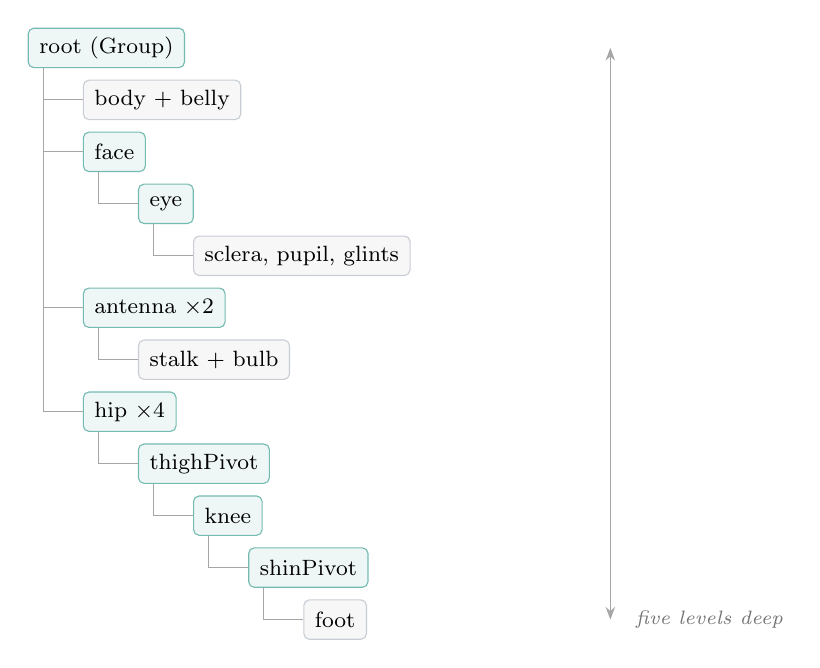
\begin{tikzpicture}[
  font=\footnotesize,
  nd/.style={draw=accent!60,fill=accent!7,rounded corners=2pt,inner xsep=4pt,inner ysep=2.5pt,
             anchor=west,minimum height=5mm},
  lf/.style={draw=rulegray,fill=black!3,rounded corners=2pt,inner xsep=4pt,inner ysep=2.5pt,
             anchor=west,minimum height=5mm},
  ln/.style={draw=black!35}
]
\def\rowsep{6.6mm}
\def\ind{7mm}
% level 0
\node[nd] (root) at (0,0) {root \textnormal{(Group)}};
% column x positions
\node[lf] (body)  at (\ind, -1*\rowsep) {body + belly};
\node[nd] (face)  at (\ind, -2*\rowsep) {face};
\node[nd] (eye)   at (2*\ind, -3*\rowsep) {eye};
\node[lf] (eyep)  at (3*\ind, -4*\rowsep) {sclera, pupil, glints};
\node[nd] (ant)   at (\ind, -5*\rowsep) {antenna $\times 2$};
\node[lf] (antp)  at (2*\ind, -6*\rowsep) {stalk + bulb};
\node[nd] (hip)   at (\ind, -7*\rowsep) {hip $\times 4$};
\node[nd] (thigh) at (2*\ind, -8*\rowsep) {thighPivot};
\node[nd] (knee)  at (3*\ind, -9*\rowsep) {knee};
\node[nd] (shin)  at (4*\ind, -10*\rowsep) {shinPivot};
\node[lf] (foot)  at (5*\ind, -11*\rowsep) {foot};

% elbow connectors: vertical drop from parent's left edge + horizontal into child
\foreach \p/\c in {root/body, root/face, root/ant, root/hip}
  { \draw[ln] ([xshift=2mm]\p.south west) |- (\c.west); }
\draw[ln] ([xshift=2mm]face.south west)  |- (eye.west);
\draw[ln] ([xshift=2mm]eye.south west)   |- (eyep.west);
\draw[ln] ([xshift=2mm]ant.south west)   |- (antp.west);
\draw[ln] ([xshift=2mm]hip.south west)   |- (thigh.west);
\draw[ln] ([xshift=2mm]thigh.south west) |- (knee.west);
\draw[ln] ([xshift=2mm]knee.south west)  |- (shin.west);
\draw[ln] ([xshift=2mm]shin.south west)  |- (foot.west);

% depth annotation
\node[font=\scriptsize\itshape,color=black!55,anchor=west] at (7.6,-11*\rowsep) {five levels deep};
\draw[{Stealth[length=1.6mm]}-{Stealth[length=1.6mm]},draw=black!35]
  (7.4,0) -- (7.4,-11*\rowsep);
\end{tikzpicture}
\captionof{figure}{The Grazer's transform hierarchy. Rotating \code{thighPivot} carries
the knee, the shin and the foot with it; rotating \code{shinPivot} carries only the
foot. Depth from root to foot is five levels.}
\end{center}

\paragraph{Welded joints by construction.} The subtlety in building an articulated limb
from primitives is that a \code{CylinderGeometry} is generated centred on the origin and
aligned with $+y$, which is the wrong frame for a bone. Rotating such a mesh about a
joint would swing it about its middle. The geometry is therefore baked into the correct
frame \emph{once}, at build time:

\begin{lstlisting}
const thighGeo = new THREE.CylinderGeometry(0.2, 0.16, L1, 10);
thighGeo.rotateZ(-Math.PI/2);     // lie along +x instead of +y
thighGeo.translate(L1/2, 0, 0);   // span 0..L1, so the joint is at the origin
\end{lstlisting}

\noindent Now each segment spans $0 \dots L$ along its local $+x$ with its pivot at the
local origin, and the next joint is simply a child \code{Group} at $(L,0,0)$:

\begin{lstlisting}
const knee = new THREE.Group(); knee.position.set(L1,0,0); thighPivot.add(knee);
\end{lstlisting}

\noindent Because the knee is a \emph{child} of the thigh's pivot, it inherits every
rotation of the thigh automatically. The segments cannot come apart --- not because the
animation is careful to keep them together, but because the hierarchy makes separation
unrepresentable. This is the whole point of hierarchical modelling, and it is why the
geometry pre-transform is worth the two extra lines.

The four hips are placed on the body surface at radius $2.45$ (greater than the body's
$2.6\times$ scaled radius at that height) and rotated so that each limb's local $+x$
points radially outward, so thighs sweep away from the body and never intersect it.

\paragraph{Solid body.} The Grazer is not a ghost. After integration, particles found
inside its bounding radius are projected onto the surface and given an outward impulse:

\begin{lstlisting}
const bR = cBodyR + psize[i];              // creature radius + particle radius
if(dd2 < bR*bR && dd2 > 1e-6){
  const d=Math.sqrt(dd2), nx=ddx/d, ny=ddy/d, nz=ddz/d;
  px[i]=cx+nx*bR; py[i]=cy+ny*bR; pz[i]=cz+nz*bR;   // project onto the surface
  const vn = vx[i]*nx + vy[i]*ny + vz[i]*nz;
  if(vn<0){ const j=-vn*1.4; vx[i]+=nx*j; vy[i]+=ny*j; vz[i]+=nz*j; }
}
\end{lstlisting}

\noindent The impulse $-1.4\,v_n$ leaves a residual normal velocity of $-0.4\,v_n$,
i.e.\ a restitution of $0.4$. The \code{vn<0} test applies the impulse only to particles
actually moving \emph{into} the surface, without which a particle sliding along the
surface would be repeatedly kicked. The collision proxy is a sphere, not the visual
mesh --- exact per-triangle collision against an articulated body would cost more than
the entire rest of the frame, and at this scale the difference is imperceptible.

\subsection{Procedural gait}
\label{sec:gait}

The walk cycle is a closed-form function of a phase accumulator. There is no keyframe
data anywhere.

\begin{lstlisting}
const gaitSpeed = 5 + moving*0.5;      // legs cycle faster when moving faster
c.phase += dt*gaitSpeed;
for(const leg of c.legs){
  const ph = c.phase + leg.phase;      // per-leg constant offset
  const lift  = Math.max(0, Math.sin(ph));   // half-wave: stance vs swing
  const swing = Math.cos(ph);
  leg.thighPivot.rotation.z =  0.18 + swing*0.24 - lift*0.10;
  leg.thighPivot.rotation.y =  swing*0.16;
  leg.shinPivot.rotation.z  = -1.7 + lift*0.5;
}
\end{lstlisting}

Each leg $k$ carries a constant phase offset $2\pi k/4$, so the four legs are evenly
distributed around the cycle and the gait reads as a coordinated walk rather than four
independent twitches. The half-wave rectification $\max(0,\sin)$ is what distinguishes
the two halves of the cycle: during swing ($\sin > 0$) the leg lifts, and during stance
($\sin \le 0$) \code{lift} is pinned to zero so the foot stays planted --- a lift term
of $\sin$ alone would make the leg burrow into the ground on the downstroke. The
constant $-1.7$ radians on the shin is the resting knee bend that gives the silhouette
its insect-like character.

\code{gaitSpeed} is tied to the creature's speed, so the legs cycle faster when the user
accelerates. This is a crude one-way coupling rather than true foot-locking, but it
removes almost all of the "skating" impression for a single multiplication.

Three secondary motions layer on top, all closed-form: a hover bob
($\sin(2.2t)$ on the root), springy antennae that lean back in proportion to speed
(\code{lean = min(0.5, moving*0.02)}), and a stochastic blink implemented as a countdown
that squashes the eye's $y$ scale for $140$\,ms and then re-arms at a random interval of
$2.5$--$5$\,s. Heading is not snapped but critically damped toward the target,
\code{rotation.y += (heading - rotation.y)*min(1, dt*6)}, so turns ease instead of
popping.

\subsection{The creature's force field}

Within a radius $R$ the Grazer applies a quadratic-falloff radial force plus a
tangential swirl:

\begin{equation}
\mathbf{a} \mathrel{+}= \underbrace{\sigma\,S\,\frac{(1-d/R)^2}{d}\,\mathbf{d}}_{\text{attract/repel}}
\;+\;
\underbrace{0.25\,S\,\frac{(1-d/R)}{d}\,(-d_z,\,0,\,d_x)}_{\text{swirl about }y}
\end{equation}

\noindent with $\sigma = \pm 1$ the mode and $S$ the strength slider. The quadratic
falloff makes the field vanish smoothly at $r=R$ rather than cutting off with a
discontinuity that would be visible as a hard shell. The swirl term is the reason
gathered particles orbit the creature instead of piling into a static ball --- it
converts pure radial infall into an accretion disc, which is far more legible as motion.
The aura sphere drawn around the creature is scaled to exactly $R$, so the visible
bubble is an honest depiction of the field's reach, and its colour tracks the mode (cool
blue for attract, warm orange for repel).

\subsection{Visualising the invisible}
\label{sec:viz}

Three optional visualisations expose structure that is normally internal.

\paragraph{Octree wireframe.} A recursive walk emits the twelve edges of each occupied
node's cube into a \code{BufferGeometry}, capped at depth 6 (deeper levels are visually
indistinguishable and expensive to emit). Empty leaves are skipped. The result makes the
Barnes--Hut adaptivity immediately obvious: cells are large and sparse in empty space and
subdivide finely exactly where mass concentrates.

\paragraph{Gravitational field streamlines.} The field is sampled on an
$n \times n \times n$ lattice ($n$ = \code{fieldN}, up to $20^3 = 8000$ samples) via
\code{gravityAccelAt}. Each sample is drawn as \emph{two} line segments sharing a
geometry: a faint full-length vector showing structure, and a bright pulse that streams
along it toward the mass. The pulse is parameterised by a travelling wave

\begin{lstlisting}
let f = ((t*speed + FLD.ph[k]) % 1 + 1) % 1;   // 0..1 travel parameter
const glow = (0.45 + 0.55*Math.sin(f*Math.PI)) * (0.5 + 0.5*s);
\end{lstlisting}

\noindent where the per-sample phase offset \code{FLD.ph[k]} is a linear function of
position, $0.05x + 0.045y + 0.04z$. Because the coefficients are unequal and
irrationally related, the resulting wave sweeps diagonally across the volume and never
resynchronises into a distracting pulse-in-unison. Colour interpolates teal $\to$ orange
with field strength, magnitudes are normalised against the frame's maximum, and samples
below $4\%$ strength are collapsed to a degenerate point rather than culled --- keeping
the vertex count constant so the buffer is never reallocated. Rendering uses additive
blending with \code{depthWrite:false}, so overlapping streamlines accumulate brightness
instead of z-fighting.

The sample \emph{directions} are rebuilt only every fourth frame (\code{vizTick\&3}),
while the pulse is redrawn every frame. This is the key optimisation: the expensive part
(8000 octree traversals) runs at 15\,Hz, while the cheap part (writing 8000 line
positions) runs at 60\,Hz, and the eye cannot tell.

\paragraph{Deforming space lattice.} A $9^3$ grid of nodes, connected into a wireframe
by $\sim 1{,}944$ segments, is displaced from its rest position by the local
gravitational acceleration (scaled $\times 7$) and by the user's active poke field, with
the total displacement capped at $9$ units so that a violent warp bends space instead of
shredding the lattice. Rest positions are stored separately from current positions, so
the deformation is always computed from the undeformed state and never accumulates
drift. This is the most direct answer to "what is gravity doing to space?" that the
application offers, and it is the intended companion to the Warp tool.

\subsection{The frame loop}

\begin{lstlisting}
function frame(now){
  const rdt = Math.min(0.05, (now-last)/1000); last=now;
  let octRoot = -1;
  if(CFG.running) octRoot = simulate(1/60*Math.min(2, rdt*60));   // physics
  pilot(rdt);                        // read keyboard, move creature
  animateCreature(rdt, t);           // gait, antennae, blink, aura
  syncMesh();                        // particles -> instance matrices
  if((CFG.showField||CFG.showLattice) && CFG.gravity && octRoot<0) octRoot = buildOctree();
  ...                                // visualisations
  if(CFG.follow && creature.root) cam.target.lerp(creature.root.position, 0.05);
  applyCam();
  renderer.render(scene, camera);
  hud.innerHTML = ...;
  requestAnimationFrame(frame);
}
\end{lstlisting}

\noindent Two details are worth pointing out. First, \code{simulate()} \emph{returns}
the octree root it built, so the visualisations can reuse it rather than rebuilding;
the tree is only constructed independently when the simulation is paused but a
visualisation still needs it. Second, the follow camera uses \code{lerp(\ldots, 0.05)}
rather than assignment, giving a critically-damped chase that lags slightly behind the
creature --- an instant snap would make the whole world jitter with the gait's hover bob.

\subsection{Performance summary}
\label{sec:perf}

\begin{center}
\small
\begin{tabular}{@{}lll@{}}
\toprule
\textbf{Stage} & \textbf{Complexity} & \textbf{Notes}\\
\midrule
Grid build            & $O(N + \text{cells})$ & Counting sort, allocation-free\\
Short-range forces    & $O(N)$ expected       & 27-cell sweep, constant density\\
Octree build          & $O(N \log N)$         & Pooled nodes, allocation-free\\
Gravity traversal     & $O(N \log N)$         & Iterative, shared explicit stack\\
Mesh sync             & $O(N)$                & One reused \code{Object3D}\\
Rendering             & 1 draw call for $N$ particles & \code{InstancedMesh}\\
Field samples         & $O(n^3 \log N)$       & Throttled to every 4th frame\\
Lattice              & $O(9^3 \log N)$        & Only when enabled\\
\bottomrule
\end{tabular}
\end{center}

\noindent The HUD exposes the live picture: frame rate, particle count, pairs evaluated
per frame, octree node count, and the current mode (\emph{chem} or \emph{2-scale}). The
steady-state allocation rate is zero, so no GC pause ever interrupts the animation.

%=============================================================================
\section{Implemented interactions}
\label{sec:interactions}
%=============================================================================

The application is interactive in five distinct registers: the user can \emph{look}
(camera), \emph{touch} (drag tools), \emph{strike} (one-shot impulses), \emph{inhabit}
(piloting the creature), and \emph{legislate} (editing the rules themselves). This
section documents each.

\subsection{Camera control}
\label{sec:orbit}

The camera is driven by a spherical orbit state, hand-written rather than taken from
three.js's \code{OrbitControls}:

\begin{lstlisting}
const cam = { target:new THREE.Vector3(0,0,0), theta:0.7, phi:1.15, radius:130 };
function applyCam(){
  const st=Math.sin(cam.phi), r=cam.radius;
  camera.position.set(
    cam.target.x + r*st*Math.sin(cam.theta),
    cam.target.y + r*Math.cos(cam.phi),
    cam.target.z + r*st*Math.cos(cam.theta));
  camera.lookAt(cam.target);
}
\end{lstlisting}

\begin{center}
\small
\begin{tabular}{@{}lll@{}}
\toprule
\textbf{Input} & \textbf{Action} & \textbf{Detail}\\
\midrule
Left-drag (Orbit tool)  & Orbit  & $\theta \mathrel{-}= 0.005\,\Delta x$, $\phi \mathrel{-}= 0.005\,\Delta y$\\
Right-drag              & Orbit  & Always orbits, whatever tool is selected\\
Middle-drag             & Pan    & Translates \code{cam.target} in the view plane\\
\keys{Shift} + left-drag & Pan   & Alternative for trackpads without a middle button\\
Scroll wheel            & Zoom   & Multiplicative, $\times 1.08$ per notch\\
One-finger drag         & Orbit  & Touch\\
Two-finger pinch        & Zoom   & Touch\\
\bottomrule
\end{tabular}
\end{center}

\noindent Several deliberate details:

\begin{itemize}[leftmargin=1.4em,itemsep=3pt]
  \item \textbf{$\phi$ is clamped} to $[0.08,\ \pi-0.08]$. Reaching the poles exactly
        makes the view direction parallel to the up vector and \code{lookAt} produces a
        degenerate basis --- the camera flips. The clamp keeps a sliver of angle in
        reserve.
  \item \textbf{Zoom is multiplicative}, not additive, and clamped to $[20,500]$. An
        additive zoom crawls when far away and overshoots through the subject when
        close; a multiplicative one feels linear at every scale.
  \item \textbf{Pan speed scales with radius} (\code{cam.radius*0.0016}), so a given
        mouse movement covers a constant fraction of the screen regardless of zoom.
  \item \textbf{Panning breaks follow mode.} If the user pans while the camera is
        following the creature, follow silently disables itself and the toggle in the
        console updates. Without this the camera would fight the user's input and lose,
        which reads as a bug rather than as a feature.
  \item \textbf{Right-drag always orbits}, so the user never becomes trapped in a tool:
        there is always a way to move the view without changing the tool selection.
        The context menu is suppressed on the canvas to make this possible.
\end{itemize}

\subsection{Direct manipulation: the drag tools}

Four tools share the left mouse button, selected in the \emph{Intervene in space}
section of the console.

\begin{center}
\small
\begin{tabular}{@{}p{1.8cm}p{12.6cm}@{}}
\toprule
\textbf{Tool} & \textbf{Effect of a left-drag}\\
\midrule
\textbf{Orbit} & Rotates the camera (the default; no effect on the simulation).\\
\textbf{Push}  & Radial outward force within the brush sphere; blasts a cavity in the soup.\\
\textbf{Pull}  & Radial inward force; gathers particles into the cursor.\\
\textbf{Warp}  & A violent composite: swirl about the view axis, inward collapse, and compression along the view axis, producing a lensing/folding effect.\\
\bottomrule
\end{tabular}
\end{center}

\paragraph{Where is the cursor in 3D?} The mouse gives a 2D position; the force needs a
3D one. We unproject the cursor onto the plane through the orbit target whose normal is
the camera's view direction --- i.e.\ the plane the user perceives as "the screen,
pushed into the scene":

\begin{lstlisting}
function screenToWorld(clientX, clientY, out){
  _ndc.x =  ((clientX-rect.left)/rect.width )*2 - 1;   // pixels -> NDC
  _ndc.y = -((clientY-rect.top )/rect.height)*2 + 1;   // (y flips)
  _ray.setFromCamera(_ndc, camera);
  camera.getWorldDirection(_n);
  _plane.setFromNormalAndCoplanarPoint(_n, cam.target);
  const r = _ray.ray.intersectPlane(_plane, _hit);
  if(r){ out.copy(_hit); return true; }
  return false;
}
\end{lstlisting}

\noindent This choice matters: because the plane is always camera-facing and passes
through the orbit target, the tool acts at the depth the user is looking at, and it
behaves identically from every viewing angle. The whole function reuses five
module-level scratch objects and allocates nothing, which matters because it runs on
every \code{mousemove}.

\paragraph{Force models.} With $d$ the distance to the poke centre, $R$ the brush
radius, $\text{fall} = 1 - d/R$, and $I$ the global intensity multiplier:

\begin{align}
\text{Push/Pull:}\quad & \mathbf{a} \mathrel{+}= \pm\,420\,I\,\frac{\text{fall}^2}{d}\,\mathbf{d}\\[4pt]
\text{Warp:}\quad & \mathbf{a} \mathrel{+}= \underbrace{620\,I\,\text{fall}^2\,(\hat{\mathbf{n}} \times \mathbf{d})}_{\text{swirl about the view axis}}
   \;\underbrace{-\;520\,I\,\frac{\text{fall}^2}{d}\,\mathbf{d}}_{\text{collapse}}
   \;\underbrace{-\;300\,I\,\text{fall}\,(\mathbf{d}\cdot\hat{\mathbf{n}})\,\hat{\mathbf{n}}}_{\text{axial compression}}
\end{align}

\noindent The swirl axis $\hat{\mathbf{n}}$ is captured as the camera's forward vector
at the moment the drag begins, so the vortex always spins in the plane of the screen ---
the user sees a whirlpool face-on rather than edge-on. The quadratic falloff again
avoids a hard edge at $r=R$. A translucent sphere with a rotating ring marks the brush
in the scene, sized to $R$ and coloured by mode (warm for push, teal for pull/warp), so
the region of influence is never guesswork.

\paragraph{Brush radius} is a slider (5--60 units); \textbf{Intensity} (0.2--6$\times$)
is a master multiplier applied to the drag tools \emph{and} to every impulse below.

\subsection{One-shot impulses}

Six buttons apply an instantaneous velocity change to every particle, centred on the
current orbit target --- i.e.\ on whatever the user is looking at. Unlike the drag
tools, these modify velocity (or, for Fold, position) directly rather than adding a
force.

\begin{center}
\small
\begin{tabular}{@{}p{1.8cm}p{12.6cm}@{}}
\toprule
\textbf{Impulse} & \textbf{Effect}\\
\midrule
\textbf{Shockwave} & Radial outward kick, $40I/(1+0.05d)$ --- an explosion whose strength decays with distance.\\
\textbf{Implode}   & Radial inward kick, $45I/(1+0.04d)$.\\
\textbf{Vortex}    & Tangential kick about the vertical axis through the epicentre, $35I$, plus a small random vertical component that keeps the disc from becoming perfectly flat.\\
\textbf{Warp}      & Swirl about the view axis combined with inward collapse, both $\propto 1/(1+0.03d)$.\\
\textbf{Fold}      & A genuine reflection of space: every particle in the far half is mirrored onto the near half, position \emph{and} velocity.\\
\textbf{Jitter}    & A uniform random kick of magnitude up to $40I$ per axis --- thermal noise, useful for shaking a structure out of a local minimum.\\
\bottomrule
\end{tabular}
\end{center}

\noindent \textbf{Fold} is the most interesting of the six because it is a
transformation of space rather than a force. Taking $\hat{\mathbf{n}}$ as the view axis
and $a = \mathbf{d}\cdot\hat{\mathbf{n}}$ the signed distance from the fold plane, every
particle with $a>0$ is reflected:

\begin{lstlisting}
if(along>0){
  px[i]-=2*along*ax; py[i]-=2*along*ay; pz[i]-=2*along*az;   // mirror position
  const vn = vx[i]*ax + vy[i]*ay + vz[i]*az;
  vx[i]-=2*vn*ax; vy[i]-=2*vn*ay; vz[i]-=2*vn*az;            // mirror velocity
}
\end{lstlisting}

\noindent Reflecting the velocity as well as the position is what makes the result
coherent: a mirrored particle continues along the mirrored trajectory, so folding a
rotating galaxy produces two counter-rotating halves that then interact --- rather than
a pile of particles moving in incoherent directions.

\subsection{Piloting the Grazer}

\begin{center}
\small
\begin{tabular}{@{}ll@{}}
\toprule
\textbf{Key} & \textbf{Action}\\
\midrule
\keys{W} / \keys{S}  & Move forward / backward along the creature's heading\\
\keys{A} / \keys{D}  & Strafe left / right, \emph{and} turn the heading ($\pm 1.8$ rad/s)\\
\keys{Q} / \keys{E}  & Ascend / descend\\
\keys{Shift}         & Boost ($2.2\times$ acceleration)\\
\keys{H}             & Show/hide the control console\\
\bottomrule
\end{tabular}
\end{center}

\noindent Movement is force-based rather than positional. The input assembles an
acceleration in the creature's local frame, which is then integrated with heavy
exponential damping:

\begin{lstlisting}
if(active){
  if(keys['a']||keys['d']) c.heading += (keys['d']?-1:1)*dt*1.8;
  accel.normalize().multiplyScalar(60*boost);
}
c.vel.addScaledVector(accel, dt);
c.vel.multiplyScalar(Math.pow(0.02, dt));    // strong damping, framerate-independent
c.root.position.addScaledVector(c.vel, dt);
c.root.position.clamp(min, max);             // stay inside the world
\end{lstlisting}

\noindent The \code{normalize()} before scaling is what stops diagonal movement from
being $\sqrt{2}$ times faster than axis-aligned movement --- the classic bug. The damping
uses the same framerate-independent exponential form as the particle friction. The
result has weight: the creature accelerates and coasts rather than teleporting, which
also means it stirs the soup as it goes.

A hint bar listing the controls fades in whenever the creature is moving and fades out
when it stops, so the controls are discoverable without a permanent overlay.

\paragraph{Follow camera.} A toggle makes \code{cam.target} chase the creature's
position each frame with a $5\%$ lerp. As noted above, panning cancels it.

\subsection{Editing the rules: the attraction matrix}

The most consequential interaction in the application is also the smallest widget. The
matrix editor is a $T \times T$ grid of coloured cells with a row and column header of
type swatches; \textbf{rows act on columns}, so cell $(i,j)$ is the force type $i$ feels
toward type $j$.

\begin{itemize}[leftmargin=1.4em,itemsep=3pt]
  \item \textbf{Colour encodes value}: green for attraction, red for repulsion,
        near-black for neutral, with the channel intensity proportional to $|A_{ij}|$.
  \item \textbf{Clicking a cell cycles} it through five discrete values:
        $+1 \to +0.5 \to 0 \to -0.5 \to -1 \to +1$. The implementation snaps to the
        nearest step first, so a cell holding a random value like $0.37$ from
        \emph{Reroll} still cycles sensibly.
  \item \textbf{Changes are instantaneous}: \code{A} is read directly by the force
        kernel every frame, so the soup reorganises as the user clicks --- no apply
        button, no reseed.
  \item \textbf{A tooltip} reports the exact value, e.g.\ \code{type 2 -> 3 (-0.50)}.
\end{itemize}

\noindent The asymmetry is the pedagogical point, and the editor is built to make it
discoverable: setting $A_{01} = +1$ and $A_{10} = -1$ --- one click each --- makes type 0
chase type 1 while type 1 flees, and the pair immediately begins to self-propel across
the volume. Making the matrix symmetric instead produces static clumps. A user can find
this out in ten seconds without reading anything.

\subsection{The control console}

The console is a collapsible panel of nine groups, all collapsed by default so that the
interface is not a wall of sliders. Every control carries a one-line explanation
underneath it. It is built by a small widget factory (\code{slider}, \code{toggle},
\code{btn}, \code{group}, \code{withDesc}) --- around 30 lines of DOM code that replaces
a UI dependency.

\begin{center}
\small
\renewcommand{\arraystretch}{1.15}
\begin{tabular}{@{}p{3.1cm}p{4.0cm}p{7.4cm}@{}}
\toprule
\textbf{Group} & \textbf{Control} & \textbf{Effect}\\
\midrule
\textbf{Simulation} & Run / Pause & Freezes physics; rendering and camera stay live\\
                    & Reset       & Re-scatters particles, keeps the rules\\
                    & Reroll      & New random rule matrix, keeps the particles\\
\midrule
\textbf{Attraction rules} & The $T\times T$ matrix & See \S6.5\\
\midrule
\textbf{Chemistry}  & Force strength (0.2--8)      & Overall power of the type rules\\
                    & Interaction radius (3--20)   & $r_{\max}$; rebuilds the grid live\\
                    & Repulsion core (0.05--0.6)   & $\beta$; incompressibility\\
                    & Friction half-life (0.01--0.2) & Damped and syrupy $\to$ lively\\
\midrule
\textbf{Gravity}    & Enable gravity     & Switches the HUD to \emph{2-scale} mode\\
                    & Strength $G$ (0--4) & \\
                    & $\theta$ (0.2--1.6) & Barnes--Hut accuracy $\leftrightarrow$ speed\\
                    & Softening (0.5--6)  & Stability at close range\\
                    & Show octree         & Draws the subdivision\\
                    & Show gravity field  & Animated streamlines\\
                    & Field density (3--20) & Samples per axis ($n^3$ total)\\
\midrule
\textbf{Population} & Particles (200--3000) & Reallocates buffers on release\\
                    & Types (2--8)          & Resizes the matrix and reseeds types\\
                    & Size variance (0--1)  & Uniform $\to$ highly varied masses\\
\midrule
\textbf{Intervene}  & Intensity (0.2--6$\times$) & Master multiplier for all interventions\\
                    & Tool: Orbit/Push/Pull/Warp & Left-drag behaviour\\
                    & Brush radius (5--60)       & \\
                    & Six impulse buttons        & See \S6.3\\
\midrule
\textbf{World \& render} & World size (40--160)  & Rescales positions and rebuilds the cage\\
                    & Wrap edges (torus)         & Periodic boundaries + minimum image\\
                    & Accent point lights        & The teal/pink pair\\
                    & Show space lattice         & Deforming wireframe of space\\
\midrule
\textbf{Grazer}     & Show creature       & Also disables its force field\\
                    & Follow camera       & \\
                    & Field: Attract/Repel & Aura colour follows the mode\\
                    & Field radius (6--40) & Matches the visible aura\\
                    & Field strength (0--400) & 0 = harmless wanderer\\
\midrule
\textbf{Presets}    & Nine one-click regimes & See \S6.8\\
\bottomrule
\end{tabular}
\end{center}

\paragraph{Live reconfiguration.} Several of these controls rebuild live state, which is
where the interesting engineering hides:

\begin{itemize}[leftmargin=1.4em,itemsep=3pt]
  \item \textbf{Particle count} reallocates all nine typed arrays, the octree pool and
        the grid, then reseeds and rebuilds the \code{InstancedMesh} (whose instance
        count is fixed at construction). It is bound to the \code{change} event rather
        than \code{input}, so it fires once when the slider is released instead of on
        every pixel of the drag.
  \item \textbf{Interaction radius} changes the grid cell size, so \code{rebuildGridDims()}
        runs on every slider step --- cheap, since it only reallocates index arrays.
  \item \textbf{World size} is the subtlest: rather than clipping particles into the new
        volume, it \emph{scales all positions} by the ratio of new to old half-width, so
        structures survive the resize instead of being crushed at the walls. The cage and
        the lattice are then rebuilt.
\end{itemize}

\subsection{Presets}

Nine presets reconfigure the rules, gravity and size distribution in one click. Each is
a genuinely different regime rather than a cosmetic variation:

\begin{center}
\small
\begin{tabular}{@{}llllll@{}}
\toprule
\textbf{Preset} & \textbf{Types} & \textbf{Gravity} & \textbf{$r_{\max}$} & \textbf{Strength} & \textbf{Character}\\
\midrule
Cells    & 5 & off & 10 & 3.2 & Soft membrane-like blobs\\
Chase    & 4 & off & 12 & 4.5 & Asymmetric hunting, moving trails\\
Galaxies & 3 & $G=1.6$ & 8  & 1.5 & Spiral, orbiting clumps\\
Web      & 6 & off & 9  & 3.8 & Connected filament network\\
Orbits   & 3 & $G=2.4$ & 6  & 0.9 & Slow stable orbits\\
Worms    & 3 & off & 14 & 5.0 & Wriggling chains\\
Crystal  & 4 & off & 8  & 2.6 & Rigid lattice-like solid\\
Nebula   & 5 & $G=0.7$ & 11 & 2.2 & Diffuse swirling clouds\\
Swarm    & 3 & off & 13 & 4.2 & Flocking drift\\
\bottomrule
\end{tabular}
\end{center}

\noindent Each preset also sets $\beta$, the friction half-life and the size variance,
rerolls the matrix, reseeds, and rebuilds the panel so every slider reflects the new
state. Because the matrix is rerolled, clicking the same preset twice gives two
different worlds \emph{of the same character} --- the preset fixes the regime, not the
outcome.

%=============================================================================
\section{User manual}
\label{sec:manual}
%=============================================================================

\subsection{Running the application}

\begin{enumerate}[leftmargin=1.6em,itemsep=3pt]
  \item Open \file{index.html} in any modern browser --- double-clicking the file is
        enough; no server, no installation, no build step.
  \item An internet connection is needed the first time, to fetch three.js from the
        CDN. To work fully offline, download \code{three.min.js} and change the first
        \code{<script src>} in \file{index.html} to point at the local copy.
  \item The simulation starts running immediately with 1000 particles, 5 types, a random
        rule matrix and gravity off.
\end{enumerate}

\subsection{The screen}

\begin{itemize}[leftmargin=1.4em,itemsep=3pt]
  \item \textbf{Left} --- the control console. Click a section header to expand it; click
        \keys{$\blacktriangleleft$} (or press \keys{H}) to hide the whole panel, and the
        \keys{$\equiv$} tab to bring it back.
  \item \textbf{Top right} --- the HUD: frame rate, particle count, pairs evaluated per
        frame, octree node count, and the current mode (\emph{chem} = chemistry only,
        \emph{2-scale} = chemistry + gravity).
  \item \textbf{Bottom centre} --- the pilot hint bar, which appears while the Grazer is
        moving.
  \item \textbf{Centre} --- the simulation, inside a faint wireframe cage marking the
        world boundary.
\end{itemize}

\subsection{Quick reference}

\begin{center}
\small
\begin{tabular}{@{}ll@{}}
\toprule
\textbf{Input} & \textbf{Action}\\
\midrule
Left-drag           & Orbit (or use the active tool)\\
Right-drag          & Orbit (always)\\
Middle-drag / \keys{Shift}+left-drag & Pan\\
Scroll              & Zoom\\
\keys{W}\keys{A}\keys{S}\keys{D} & Pilot the Grazer\\
\keys{Q} / \keys{E} & Grazer up / down\\
\keys{Shift}        & Boost\\
\keys{H}            & Toggle the console\\
One finger / two fingers & Orbit / pinch-zoom\\
\bottomrule
\end{tabular}
\end{center}

\subsection{A guided tour}

The following sequence takes about ten minutes and exercises every subsystem.

\begin{enumerate}[leftmargin=1.6em,itemsep=5pt]
  \item \textbf{Watch first.} Let the default random matrix run for thirty seconds and
        orbit around it. Whatever structure appears was not designed --- it is the
        matrix expressing itself.

  \item \textbf{Change one rule.} Open \emph{Attraction rules} and click a single cell
        until it is bright green, then click its mirror cell until it is bright red.
        Watch those two colours begin to chase each other. This is asymmetry, and it is
        the engine of every moving pattern in the system.

  \item \textbf{Try the presets.} Open \emph{Presets} and work down the list. Compare
        \emph{Crystal} (rigid, locked) with \emph{Worms} (crawling chains) --- same code,
        same particles, different numbers.

  \item \textbf{Turn on gravity.} Click \emph{Galaxies}. The mode indicator in the HUD
        switches to \emph{2-scale}. Now enable \emph{Show octree}: the cubes are large
        in empty space and subdivide tightly around the clumps. This adaptivity is why
        the frame rate survives.

  \item \textbf{Break the octree on purpose.} With the octree visible, drag $\theta$
        from $0.8$ up to $1.6$ and watch the node count in the HUD collapse and the
        frame rate climb --- then drag it down to $0.3$ and watch the opposite. You are
        looking directly at the accuracy/speed trade-off.

  \item \textbf{See the field.} Enable \emph{Show gravity field} and raise
        \emph{Field density} to about 12. Bright pulses stream along each vector toward
        mass, with a wave sweeping diagonally across the volume.

  \item \textbf{Bend space.} Enable \emph{Show space lattice}, then select the
        \textbf{Warp} tool and drag through the middle of a clump. The lattice twists and
        collapses around the cursor. Raise \emph{Intensity} to $4\times$ and try again.

  \item \textbf{Fold the universe.} Click \emph{Fold}. The far half of space is mirrored
        onto the near half; the two halves then collide and interact.

  \item \textbf{Go for a swim.} Set \emph{Field: Attract}, \emph{Field strength} to
        $\sim300$, enable \emph{Follow camera}, and pilot with \keys{W}\keys{A}\keys{S}\keys{D}.
        Particles gather into an orbiting disc around the Grazer and are dragged along
        behind it. Switch to \emph{Repel} to plough a tunnel through the soup instead.

  \item \textbf{Push the limits.} Raise \emph{Particles} to 3000 and watch the HUD. If
        the frame rate drops, raise $\theta$, lower the field density, or turn off the
        visualisations --- and note which one buys the most.
\end{enumerate}

\subsection{Troubleshooting}

\begin{center}
\small
\begin{tabular}{@{}p{5.0cm}p{9.5cm}@{}}
\toprule
\textbf{Symptom} & \textbf{Cause and remedy}\\
\midrule
Black screen, nothing renders & three.js failed to load from the CDN. Check the network, or switch to a local copy of \code{three.min.js}.\\
Low frame rate & Lower \emph{Particles}; raise $\theta$; lower \emph{Field density}; disable the octree/field/lattice visualisations.\\
Everything collapses to a dot & $G$ too high or \emph{Repulsion core} too low. Raise $\beta$, lower $G$, or raise \emph{Softening}.\\
Particles fly apart violently & \emph{Force strength} or \emph{Intensity} too high; friction half-life too long. The velocity clamp prevents a true explosion but the result is still noise.\\
Nothing happens when I drag & The active tool is \emph{Orbit}. Select Push, Pull or Warp --- or just use right-drag to orbit.\\
The camera will not follow & Follow mode disables itself whenever you pan. Re-enable it in the \emph{Grazer} section.\\
No creature visible & \emph{Show creature} is off, or it has been piloted out of view. Enable \emph{Follow camera} to find it.\\
\bottomrule
\end{tabular}
\end{center}

%=============================================================================
\section{Limitations and future work}
\label{sec:limitations}
%=============================================================================

We state the limitations plainly; each is a considered trade-off rather than an
oversight.

\begin{enumerate}[leftmargin=1.6em,itemsep=4pt]
  \item \textbf{Single-threaded, CPU-bound.} The whole simulation runs on the main
        thread. Beyond roughly 3000 particles the force evaluation, not the rendering,
        is the bottleneck. The natural fixes are a Web Worker with a
        \code{SharedArrayBuffer} (which would need COOP/COEP headers, and therefore a
        server --- breaking the \code{file://} promise), or moving the integration to
        the GPU via transform feedback or a compute pass, which is a substantial rewrite.
  \item \textbf{Gravity is not periodic.} With \emph{Wrap edges} enabled, the
        short-range term uses the minimum-image convention but gravity does not: it
        still sees the non-wrapped configuration. A correct treatment needs an Ewald
        summation, which is out of scope for a real-time browser application.
  \item \textbf{The creature's collision proxy is a sphere}, not its visual silhouette.
        Particles bounce off an invisible ball rather than off the legs. Exact collision
        against an articulated body would dominate the frame budget for an effect that
        is barely perceptible at this scale.
  \item \textbf{The gait is not foot-locked.} Leg cycle speed tracks body speed, but
        feet are not constrained to be stationary while planted, so a slight skate
        remains at high speed. Proper foot-locking needs inverse kinematics.
  \item \textbf{Momentum is not conserved} --- by design. The asymmetric matrix violates
        Newton's third law, which is the entire point of the chemistry model, but it does
        mean the system has no conserved quantity to validate against.
  \item \textbf{Bodies dropped at extreme density.} The octree's coincident-body guard
        drops a particle from the tree when a cell shrinks below $0.02$ units. This
        introduces a small, bounded gravitational error in extremely dense clumps, and is
        preferable to an infinite subdivision that would hang the browser.
  \item \textbf{Instance count is fixed at construction}, so changing the particle count
        rebuilds the \code{InstancedMesh}. This causes a brief hitch, which is why the
        control fires on slider release rather than during the drag.
\end{enumerate}

\paragraph{Natural extensions.} GPU-side integration; a proper IK solver with foot
locking; multiple creatures with flocking behaviour among themselves; recording and
replaying parameter trajectories; saving and loading matrices as shareable URLs; and
soft-body or bonded-particle chains built on the existing neighbour grid.

%=============================================================================
\section{Conclusions}
%=============================================================================

\textsc{Primordia} sets out to demonstrate that complexity does not require complicated
rules. Two force laws --- a piecewise-linear typed kernel and a softened inverse-square
law --- acting at two different spatial scales are sufficient to produce cells, chains,
filaments, orbits, spirals and swarms, none of which appears anywhere in the source as
an explicit construct.

The engineering that makes this interactive rather than merely correct is the pairing of
each force law with the acceleration structure suited to its scale: a uniform grid,
valid precisely because the short-range kernel has compact support, and a Barnes--Hut
octree, valid because a distant cluster is well approximated by its centre of mass.
Both are built on pooled typed arrays, so the steady-state allocation rate is zero and
the animation is never interrupted by a garbage collection pause. The user-facing payoff
of that work is the $\theta$ slider and the octree visualisation: the approximation is
not hidden behind the curtain, it is on stage, and the user can watch the trade-off it
makes.

The project satisfies its self-imposed asset-free constraint completely: every vertex,
texel and joint angle is computed in JavaScript at run time, and the entire application
consists of one HTML file, one stylesheet and ten JavaScript files with a single
third-party dependency.

%=============================================================================
\begin{thebibliography}{9}
\bibitem{barneshut}
J.~Barnes and P.~Hut,
\emph{A hierarchical $O(N \log N)$ force-calculation algorithm},
Nature, vol.~324, pp.~446--449, 1986.

\bibitem{ventrella}
J.~Ventrella,
\emph{Clusters --- artificial life with simple particle interaction rules}.
\url{http://www.ventrella.com/Clusters/}

\bibitem{hunar}
H.~Ahmad (\code{hunar4321}),
\emph{Particle Life --- a simple simulation of emergent behaviour}.
\url{https://github.com/hunar4321/particle-life}

\bibitem{threejs}
three.js --- a JavaScript 3D library, revision 128.
\url{https://threejs.org}

\bibitem{aarseth}
S.~J.~Aarseth,
\emph{Gravitational N-Body Simulations: Tools and Algorithms},
Cambridge University Press, 2003. (Reference for softening and time-step stability.)
\end{thebibliography}

\end{document}
